\documentclass{report}
\usepackage{ugentstyle}



\begin{document}
	\maketitle{Systeemontwerp}
	\tableofcontents
	\chapter{Inleiding}
	\begin{itemize}
		\item[\info] \underline{Systeemontwerp} = het ontwerpen van een infrastructuur waarbij verschillende componenten met elkaar kunnen interageren.
		\item[\info] Typische high level architectuurblokken: 
			\begin{itemize}
				\item[\info] \underline{transactiebehandeling}: requests behandelen van gebruikers.
				\item[\info] \underline{business intelligence}: geproduceerde data analyseren.
			\end{itemize}  
	\end{itemize}
	\section{Softwarearchitectuur}
	\subsection{Systeemrequirements}
	\begin{itemize}
		\item[\info] \underline{functionele requirements}: specificatie wat een systeem moet \textbf{doen}.
		\item[\info] \underline{niet-functionele requirements}: specificatie wat een systeem moet \textbf{zijn} (kwaliteitseisen).
	\end{itemize}

	\subsection{4+1 view model}
	\begin{itemize}
		\item[\info] Logical view:
			\begin{itemize}
				\item[\info] Bevat de klassen, packages, relaties tussen klassen, associaties tussen de klassen (\accentuate{domain class diagram en entity-relationship diagram})
			\end{itemize}
		\item[\info] Implementation view:
			\begin{itemize}
				\item[\info] Bevat de output van het build systeem, zoals de verschillende modules (bv JARs) en componenten (executables, WARS).
				\item[\info] Beschrijft de onderliggende relaties tussen alle modules en componenten (import, use, merge, ...)
			\end{itemize}
		\item[\info] Process view:
			\begin{itemize}
				\item[\info] Bevat de beschrijving van de werking van verschillende processen (een proces kan een hele module zijn) (\accentuate{activity diagram}).
				\item[\info] Een proces kan beheerd worden: starten, pauzeren, configureren, stoppen.
				\item[\info] Heeft als doel om \underline{deadlocks} en \underline{netwerkvertragingen} te voorkomen en \underline{consistentie} te bereiken. 
			\end{itemize}
		\item[\info] Deployment view:
			\begin{itemize}
				\item[\info] Beschrijft op welke toestellen de processen moeten gedeployed worden, hoeveel toestellen er gebruikt worden.
				\item[\info] Verschillende deploymentconfiguraties mogelijk per klant of geografisch gebied, maar ook of dat het een productie of ontwikkelomgeving is.
			\end{itemize}
		\item[\info] \accentuate{+1} Use Cases/Scenarios:
			\begin{itemize}
				\item[\info] Een use case beschrijft, binnen een view, hoe dat de componenten binnen die view met elkaar interageren voor een bepaalde situatie.
				\item[\info] Is eigenlijk redundant omdat andere 4 views deze informatie ook al bevatten, maar \underline{use cases zijn toch nuttig}:
				\begin{itemize}
					\item[\good] Het valideert het ontwerp.
					\item[\good] Het kan nieuwe systeemelementen ontdekken.
				\end{itemize}
			\end{itemize}
	\end{itemize}
	\section{Reactive manifesto}
	\underline{4 kenmerken:}
	\begin{itemize}
		\item[\info] Message Driven: asynchrone communicatie tussen componenten. Maakt gebruik van een wachtrij om de berichten te beheren. Dit heeft \underline{drie voordelen}:
		\begin{itemize}
			\item[\good] Zwakke koppeling: de verschillende componenten moeten enkel een protocol afspreken voor het bericht. 
			\item[\good] Loskoppelen van de tijd: Zender en ontvanger moeten niet wachten op elkaar.
			\item[\good] Loskoppelen van locatie: De zender en ontvanger moeten niet in hetzelfde proces beschikbaar zijn, enkel de locator (\accentuate{analogie met gsm-nummer, ik kan eender waar naar iemand bellen, onafhankelijk van zijn locatie}) moet bekend zijn.
		\end{itemize}
		\item[\info] Responsief:
			\begin{itemize}
				\item[\info] Lazy loading
				\item[\info] Toon progressbar
				\item[\info] Een trage service mag andere services niet beïnvloeden.
			\end{itemize}
		\item[\info] Elastisch:
			\begin{itemize}
				\item[\info] Predictieve en reactieve schaling
				\item[\info] Resources moeten voor elk individueel component instelbaar zijn
				\item[\info] Systeem moet responsief blijven
			\end{itemize}
		\item[\info] Foutbestendig:
			\begin{itemize}
				\item[\info] Systeem moet zichzelf kunnen herstellen
				\item[\info] Fouten moeten snel opgespoord kunnen worden via monitoring
				\item[\info] Voorzie fallback services
			\end{itemize}
	\end{itemize}

	\part{Microservices}
	\chapter{Architectuurstijlen}
	\begin{itemize}
		\item[\info] Gelaagde stijl:
		\begin{itemize}
			\item[\info] Kan toegepast worden op elk view model.
			\item[\info] 3 lagen in het \textbf{logische view}: persistentie, presentatie en domeinlogica.
			\item[\good] Robust systeem.
			\item[\good] Eenvoudig om te ontwikkelen (veel frameworks ondersteunen dit: Java EE, .NET, ...).
			\item[\good] De verschillende lagen kunnen gemockt worden om eenvoudig testen uit te voeren.
			\item[\alert] Slechts één presentatielaag, maar er kunnen verschillende clients zijn (desktop, mobile, tablet, ...).
			\item[\alert] Slechts één persistentielaag, maar er kunnen verschillende databasetechnologiën gebruikt worden.
			\item[\alert] De domeinlogicalaag definieert repositories, maar de persistentielaag implementeert deze. De dependency is dus omgekeerd.
		\end{itemize}
		\item[\info] Hexagonale stijl:
		\begin{itemize}
			\item[\info] Maakt gebruik van adapters. Deze adapters zijn interfaces en kunnen opgesplitst worden:
			\begin{itemize}
				\item[\info] \textbf{Inbound adapter}: Dit is API dat de domeinlogica openstelt, zodat deze kan aangeroepen worden door externen. Elke client kan nu onafhankelijk van elkaar ontwikkeld worden. Ze moeten enkel maar de API aanroepen.
				\item[\info] \textbf{Outbound adapter}: Dit is de API die de domeinlogica kan gebruiken (repository interface, payment interface).
			\end{itemize}
			\item[\good] presentatie-, persistentie- en domeinlogicalaag zijn losgekoppeld.
		\end{itemize}
		\item[\info] Monolithische stijl:
		\begin{itemize}
			\item[\info] Een monolitische applicatie bevat de drie lagen van de gelaagde stijl, en verpakt dit in één executable.
			\item[\good] Makkelijk te ontwikkelen met een IDE.
			\item[\good] Eenvoudig om wijzigingen door te voeren: edit $\rightarrow$ build $\rightarrow$ deploy.
			\item[\good] Eenvoudig te testen.
			\item[\good] Eenvoudig om te deployen.
			\item[\alert] Voor grote codebases wordt het moeilijk om elk detail van de codebase te kennen.
			\item[\alert] Een kleine wijziging resulteert in het rebuilden van de hele applicatie.
			\item[\alert] Een bug kan het hele systeem onbereikbaar maken.
			\item[\alert] Replicatie is haast onmogelijk. 
		\end{itemize}
		\item[\info] \textbf{Microservices}:
		\begin{itemize}
			\item[\info] Decomposeerd een applicatie in kleine, zwak gekoppelde services, die individueel kunnen gedeployed worden.
			\item[\info] Services communiceren met elkaar via APIs.
			\item[\info] Wordt geïmplementeerd in de implementatie view. Elke service heeft zijn eigen logische view.
			\item[\info] \underline{Wat is een service?}
			\begin{itemize}
				\item[\info] Een individueel component dat een bepaalde functionaliteit aanbiedt.
				\item[\info] Deze functionaliteit wordt via een API beschikbaar gesteld. 
			\end{itemize}
			\item[\info] \underline{Wat is een service?}
			\begin{itemize}
				\item[\info] Een service dat goed gedefinieerd is in functie van de business.
				\item[\info] Voert een eenvoudige functie uit, en kan door een klein ontwikkelteam beheerd worden.
			\end{itemize}
			\item[\alert] De juiste services vinden is moeilijk.
			\item[\alert] Foute decompositie leidt tot een gedistribueerd monolitisch systeem.
			\item[\alert] Gedistribueerde systemen zijn complex. (bv geen IDE die dit ondersteund).
			\item[\alert] Communicatie tussen services (over een netwerk) is traag.
			\item[\alert] Vele verschillende services kunnen op hetzelfde moment aan het draaien zijn. 
		\end{itemize}
	\end{itemize}
	
	\chapter{Decompositie van een applicatie}
	Het proces om een applicatie in te delen in verschillende microservices noemt men \textbf{decompositie}. Dit \textbf{iteratief} proces is belangrijk aangezien een foutieve methode leidt tot ongewenste resultaten. Een dergerlijk proces kan opgedeeld worden in drie stappen.
	\begin{enumerate}
		\item \textbf{Identificatie van de systeemoperaties.} Dit omvat het vertalen van de noden van één of meerdere gebruikers naar user stories en use-cases. Vaak wordt er hier overlegd met enkele domeinexperts. Het is belangrijk om te achterhalen wat belangrijke systeemoperaties zijn. Welke informatie moet er met een \textit{create}, \textit{update} of \textit{delete} gewijzigd worden? Welke informatie moet met een \textit{query} opgehaald worden? In deze fase worden er nog geen technische vaststellingen gedaan. De focus ligt namelijk op het vaststellen van de pre- en postcondities van de verschillende systeemoperaties.
		
		\item \textbf{Identificatie van de services.} Services specificeren handelingen dat een bedrijf kan doen. Voorbeelden voor een online webshop zijn: \textit{Sales}, \textit{Marketing}, \textit{Payment}, \textit{Order Shipping} en \textit{Order Tracking}. Deze services blijven lang stabiel en zullen haast nooit veranderen tenzij de business een shift van focus doen. Een obstakel dat zich kan voordoen zijn \textbf{godklassen}. Dit zijn klassen die te veel verantwoordelijkheid op zich dragen. Een oplossing hiervoor is om deze klasse in een centrale databank op te slaan en services die deze klasse nodig hebben kunnen die dan via de databank aanspreken. Dit is duidelijk een overtreding op de principes van de microservice architectuur. Er is nu een sterke koppeling tussen de microservices en de godklasse. Een betere oplossing is het opsplitsen van de klasse in verschillende klassen op basis van de bestaande services. Deze verschillende klassen kunnen in een microservice gestoken worden waarbij de definitie van de klasse sterk gedaald is (ze moet maar gelden binnen de microservice). Voorbeeld van een godklasse is een \textbf{Order} klasse voor pizza's. Denk aan de typische attributen: \textit{status}, \textit{requestedDeliveryTime}, \textit{prepareByTime}, \textit{deliveryTime}, \textit{paymentinfo}, \textit{deliveryAddress}, ... . Het opsplitsen van deze klassen kan bijvoorbeeld gebeuren door enkel informatie die relevant is voor de keuken, in een keukenserivce te steken en informatie die enkel relevant is voor het bezorgen van een bepaalde order in een deliveryservice. Op die manier worden godklassen vermeden.
		
		\item \textbf{Identificatie van de service API's.} Deze laatste stap zal nagaan welke operaties van een microservice publiek moeten gesteld worden aan de buitenwereld via een API. 
	\end{enumerate}
	\chapter{Interactiestijlen tussen services}
	\begin{table}[ht]
		\centering
		\begin{tabular}{c | c | c}
			& one-to-one & one-to-many \\
			\hline
			synchroon & request/response & / \\
			\hline 
		asynchroon & \hspace{2em} \begin{minipage}[c]{0.3\textwidth}request/async response \\ one way notifications\end{minipage} & \hspace{2em} \begin{minipage}[c]{0.3\textwidth}publish/subscribe \\ publish/async response\end{minipage}
		\end{tabular}
	\end{table}
	\begin{itemize}
		\item[\info] request/response: Een service stuurt een request en wacht op een response.
		\item[\info] request/async response: Een service stuurt een request, maar wacht niet noodzakelijk op een response.
		\item[\info] one way notifications: Een service stuurt een request en verwacht geen response.
		\item[\info] publish/subscribe: Een service publiceerd een bericht en kan opgevangen worden door 0 of meerdere geïnteresseerden.
		\item[\info] publish/async responses: Een service publiceerd een bericht en zal eventueel antwoorden opvangen van 0 of meerdere geïnteresseerden.
	\end{itemize}
	\section{Synchrone communicatie}
	\underline{Voorbeelden van synchrone communicatie}: REST en gRPC.
	\begin{itemize}
		\item[\info] REST
		\begin{itemize}
			\item[\info] Vier levels:
			\begin{enumerate}
				\item[0]: Enkel HTTP POST mogelijk. Elke actie krijgt dan ook een ander endpoint toegewezen.
				\item[1]: Maakt gebruik van resources zodat elk individuele resource een URI krijgt. Nog steeds enkel HTTP POST mogelijk.
				\item[2]: GET, POST, PUT mogelijk. Een zelfde resource kan nu meerdere operaties ondersteunen.
				\item[3]: HATEEOAS mogelijk: een GET request bevat, behalve het object, ook URLs die mogelijke acties op het object toelaten.
			\end{enumerate}
			\item[\good] HTTP wordt niet geblokkeerd door een firewall.
			\item[\good] Implementeerd request/response interactie.
			\item[\alert] clients moeten de locatie (URL) kennen.
			\item[\alert] Meerdere resources in één request opvragen is moeilijk. 
			\item[\alert] Soms is het moeilijk om de HTTP werkwoorden te mappen op een operatie.
		\end{itemize}
		\item[\info] gRPC
		\begin{itemize}
			\item[\info] Google Remote Procedure Call.
			\item[\info] API wordt gedefinieerd op basis van een Interface Definition File. Dit bestand bevat IDL (Interface Description Language) code.
			\item[\info] Deze code wordt gecompileerd afhankelijk van de gekozen client.
			\item[\alert] Het valt niet op dat de communicatie nu over het netwerk gebeurd.
		\end{itemize}
	\end{itemize}
	\underline{Hoe foutbestendig maken?}

	\chapter{Saga}
	=\underline{garanderen dat een transactie ofwel volledig, ofwel niet uitgevoerd wordt.}
	\begin{itemize}
		\item[\info] Traditioneel: 2-fasen-commit.
		\begin{itemize}
			\item[\info] Eerst wordt elke databank naarwaar geschreven moet worden, op de hoogte gebracht van de informatie die ze moeten schrijven.
			\item[\info] De eerste fase zal aan elke databank vragen of zij klaar zijn om weg te schrijven (prepare-fase).
			\item[\info] De tweede fase zal effectief een commit uitvoeren op elke databank (commit-fase).
			\item[\info] Van zodra één databank 'nee' antwoord, wordt het hele proces gestopt.
			\item[\alert] Synchroon
			\item[\alert] Niet elke database implementeert het concept van transacties en locking.
		\end{itemize}
		\item[\info] \textbf{Saga}
		\begin{itemize}
			\item[\info] Een sequentie van lokale interacties tussen verschillende microservices.
			\item[\info] Elke systeemoperatie moet een saga hebben.
			\item[\info] 
		\end{itemize}
	\end{itemize}
	
	\part{Container deployment and orchestration}
	\chapter{Productieomgeving}
	Een applicatie kan over een groot aantal services beschikken, die allemaal gebruik maken van verschillende technologiën. Een service kan eigenlijk beschouwd worden als een kleine applicatie, zodat er in plaats van één grote applicatie, meerdere kleinere applicaties in productie moeten draaien. Zo een productieomgeving moet vier functionaliteiten implementeren:
	\begin{enumerate}
		\item \textbf{Service management interface.} Het in staat zijn om services te creëren, configureren en updaten, vaak via een shell of GUI.
		\item \textbf{Runtime service management.} De omgeving moet automatisch services kunnen herstarten indien deze gecrasht zijn. Ook als een fysieke server faalt, moet de omgeving een andere server aanspreken om de service op te draaien.
		\item \textbf{Monitoring.} Informatie over elke service instance zoals logbestanden en metrieken voor die bepaalde service (aantal bezoekers per seconde, sucess rate, ...) moeten beschikbaar zijn voor de ontwikkelaars, en moeten ook gewaarschuwd worden indien een service niet aan de vooropgestelde criteria voldoet.  
		\item \textbf{Request routing.} De requests dat users versturen moeten naar de juiste service doorverwezen worden.
	\end{enumerate}

	Volgende paragrafen bespreken hoe een aantal van deze zaken geïmplementeerd kunnen worden.

	Een service heeft altijd een aantal configuratiegegevens (\textbf{environment variabelen} genoemd), die afhankelijk zijn van de omgeving waarin de service draait. Een service moet zo ontworpen zijn dat deze slechts éénmaal gecompileerd moet worden door de deployment pipeline, zodat deze meerdere malen in productie gezet kan worden. Het externalizeren van de configuratiegegevens betekent dat de configuratie van een service tijdens runtime bepaalt wordt. Hier zijn er twee modellen mogelijk:
	\begin{itemize}
		\item \textbf{Push model.} Bij dit model zal de service bij het opstarten configuratiegegevens verwachten, die door de deploymentomgeving meegegeven worden. Hoe deze configuratiegegevens gegeven worden (via bestand, of individuele parameters) maakt niet uit. De service en deploymentomgeving moeten wel onderling van elkaar weten hoe de structuur van de configuratiegegevens in elkaar zit. Het \underline{grootste nadeel} van deze methode is dat een service haast niet meer gewijzigd kan worden na het initialiseren van de service. Een ander \underline{nadeel} is dat de configuratiegegevens verspreidt over de services liggen.
		\item \textbf{Pull model.} Het pull model heeft bijna enkel voordelen tegenover het push model. De deploymentomgeving geeft bij de creatie van de service enkel de URL mee van een zogenaamde \underline{configuratieserver}. Deze server bevat alle configuratiegegevens voor elke service. De service zelf zal dan deze server, met behulp van de URL, aanspreken om de juiste configuratiegegevens op te halen. Dit biedt een aantal \underline{voordelen}:
		\begin{itemize}
			\item Gecentraliseerde configuratie.
			\item Een service kan de server pollen om na te gaan of de configuratiegegevens aangepast zijn, en deze dan eventueel op te halen. De service moet hiervoor niet herstart worden.
			\item Sommige configuratiegegevens zijn gevoelig, zoals databaseinformatie. De server zal deze moeten encrypteren. De service wordt dan wel verwacht de publieke sleutel van de server te hebben zodat hij deze kan decrypteren. Sommige servers decrypteren de configuratiegegevens zelf.
		\end{itemize}
		Het \underline{grootste nadeel} is echter dat de configuratieserver opnieuw een infrastructuur is dat moet opgesteld en onderhouden worden.
	\end{itemize}

	Om \textbf{monitoring} te implementeren moeten services 'waarneembaar' gemaakt worden. Er moeten hiervoor extra APIs aangemaakt worden, die niet mogen interfereren met de werkelijke functionaliteit van de service. Hiervoor zijn er een aantal hulpmiddelen om een service waarneembaar te maken:
	\begin{itemize}
		\item \textbf{Health check API.} Een eenvoudige API dat de status van de service teruggeeft.
		\item \textbf{Log aggregation.} Logbestanden zijn een goede manier om de werking van de service op te volgen. Deze logbestanden worden best geschreven naar een gecentraliseerde logserver, zodat \underline{zoeken} ondersteund kan worden. Het is ook enkel de verantwoordelijkheid van de logserver om ontwikkelaars te waarschuwen. Traditioneel logt een applicatie naar een welbepaald logbestand op het filesysteem. Dit is hier geen goede oplossing, omdat sommige services zelfs geen filesysteem zullen hebben. Hierom moet elke service loggen naar stdout. De deploymentomgeving zal dan beslissen wat hij wil doen met deze uitvoer. 
		\item \textbf{Distributed tracing.} Het oproepen van een endpoint van de API kan meerdere interne calls maken. Het is vaak moeilijk te achterhalen waarom zo een query traag verloopt. Distributed tracing kent aan elke endpoint een ID toe, en bekijkt de call chain die overlopen wordt. Deze gegevens worden naar een gecentraliseerde server verstuurd waarop analyse kan uitgevoerdt worden. Een endpoint wordt gepresenteerd door een \underline{trace}. Zo een trace bestaat uit geneste \underline{spans}, die elk een call voorstellen. De endpoint is de top span, en zal elke andere span bevatten. 
		\item \textbf{Audit logging.} Het doel van audit logging is om acties van gebruikers te verzamelen. Elke audit log entry heeft een ID dat een gebruiker voorstelt, de actie dat ze uitgevoerd hebben en het domeinobject. Voorbeelden zijn gefaalde loginpoging, toevoegen van items in het winkelmandje, maar uiteindelijk niet betalen. Zulke logs dienen vooral voor customer support en om vreemde activiteiten op te sporen.
		\item \textbf{Application metrics.} Deze tak bestaat uit een metriekservice. Deze metriekservice vraagt gegevens op van de verschillende applicaties. Zulke gegevens zijn onder andere: CPU gebruik, geheugengebruik, schijfgebruik, aantal requests per seconde, request latency en domeinspecifieke gegevens. Een service moet ontworpen zijn zodat al deze gegevens naar de metriekservice kunnen verstuurd worden, en is afhankelijk van het gebruikte framework. De service kan ofwel zelf beslissen om zijn metrieken te versturen naar de metriekservice, of de metriekservice zal elke service pollen om de metrieken op te halen.
	\end{itemize}
	\chapter{Containers}
	Verschillende microservices kunnen onderling elk gebruik maken van verschillende technologiën. Om deze verschillende microservices te deployen zouden al de verschillende dependencies van elke technologie op de server geconfigureerd moeten worden. Dit is natuurlijk niet haalbaar op grote schaal, daarom zou men in eerste instantie virtuele machines kunnen gebruiken waarbij elke verschillende virtuele machine geshickt is voor een specifieke technologiestack. Virtuele machines nemen echter te veel opslag in beslag. Ze nemen zoveel beslag in omdat elke virtuele machine zijn eigen besturingssysteem en kernel bevat. De hypervisor (of virtual machine monitor) geeft elke virtuele machine de illusie dat enkel hun machine toegang heeft tot de resources van het \underline{hosttoestel} (het toestel waarop de virtuele machines draaien). 
	Er zijn twee types hypervisor:
	\begin{itemize}
		\item \textbf{Type 1.} Dit type hypervisor draait rechtstreeks op de hardware van de host en heeft geen behoefte aan een onderliggend besturingssysteem. 
		\item \textbf{Type 2.} Dit type hypervisor heeft wel nood aan een besturingssysteem. Dit heeft als voordeel dat er ook applicaties op het hosttoestel kunnen draaien.
	\end{itemize}
	\underline{Containers} zijn een virtualisatietechniek op besturingssysteemniveau. Een populaire container technologie is Docker, dat gebruik maakt van de linux container functionaliteit.  
	\begin{itemize}
		\item \textbf{Linux Control Groups (cgroups).} Groeperen van processen, en privileges zetten op deze groepen.
		\item \textbf{Linux namespaces.} Een geïsoleerde weergave van de systeemresources.
		\item \textbf{Changing root (chroot).} Elk process de illusie geven dat ze vanuit de root-directory aangesproken worden.
		\item \textbf{Veilige containers (LSM).} Mogelijkheden per process vastzetten.
	\end{itemize}

	\underline{Docker}:
	\begin{itemize}
		\item Automatisch verpakken en deployen van een applicatie.
		\item Beschikbaar op Linux, MacOS, Windows.
		\item Onafhankelijk. Minimale dependencies.
		\item Grote flexibiliteit in wat er in de container moet.
		\item Alle containers kunnen gestart en gestopt worden op dezelfde manier.
		\item Lightweight. Meerdere containers per host mogelijk (nog meer dan virtuele machines).
	\end{itemize}

	\section{Docker Architecture}
	\begin{figure}[ht]
		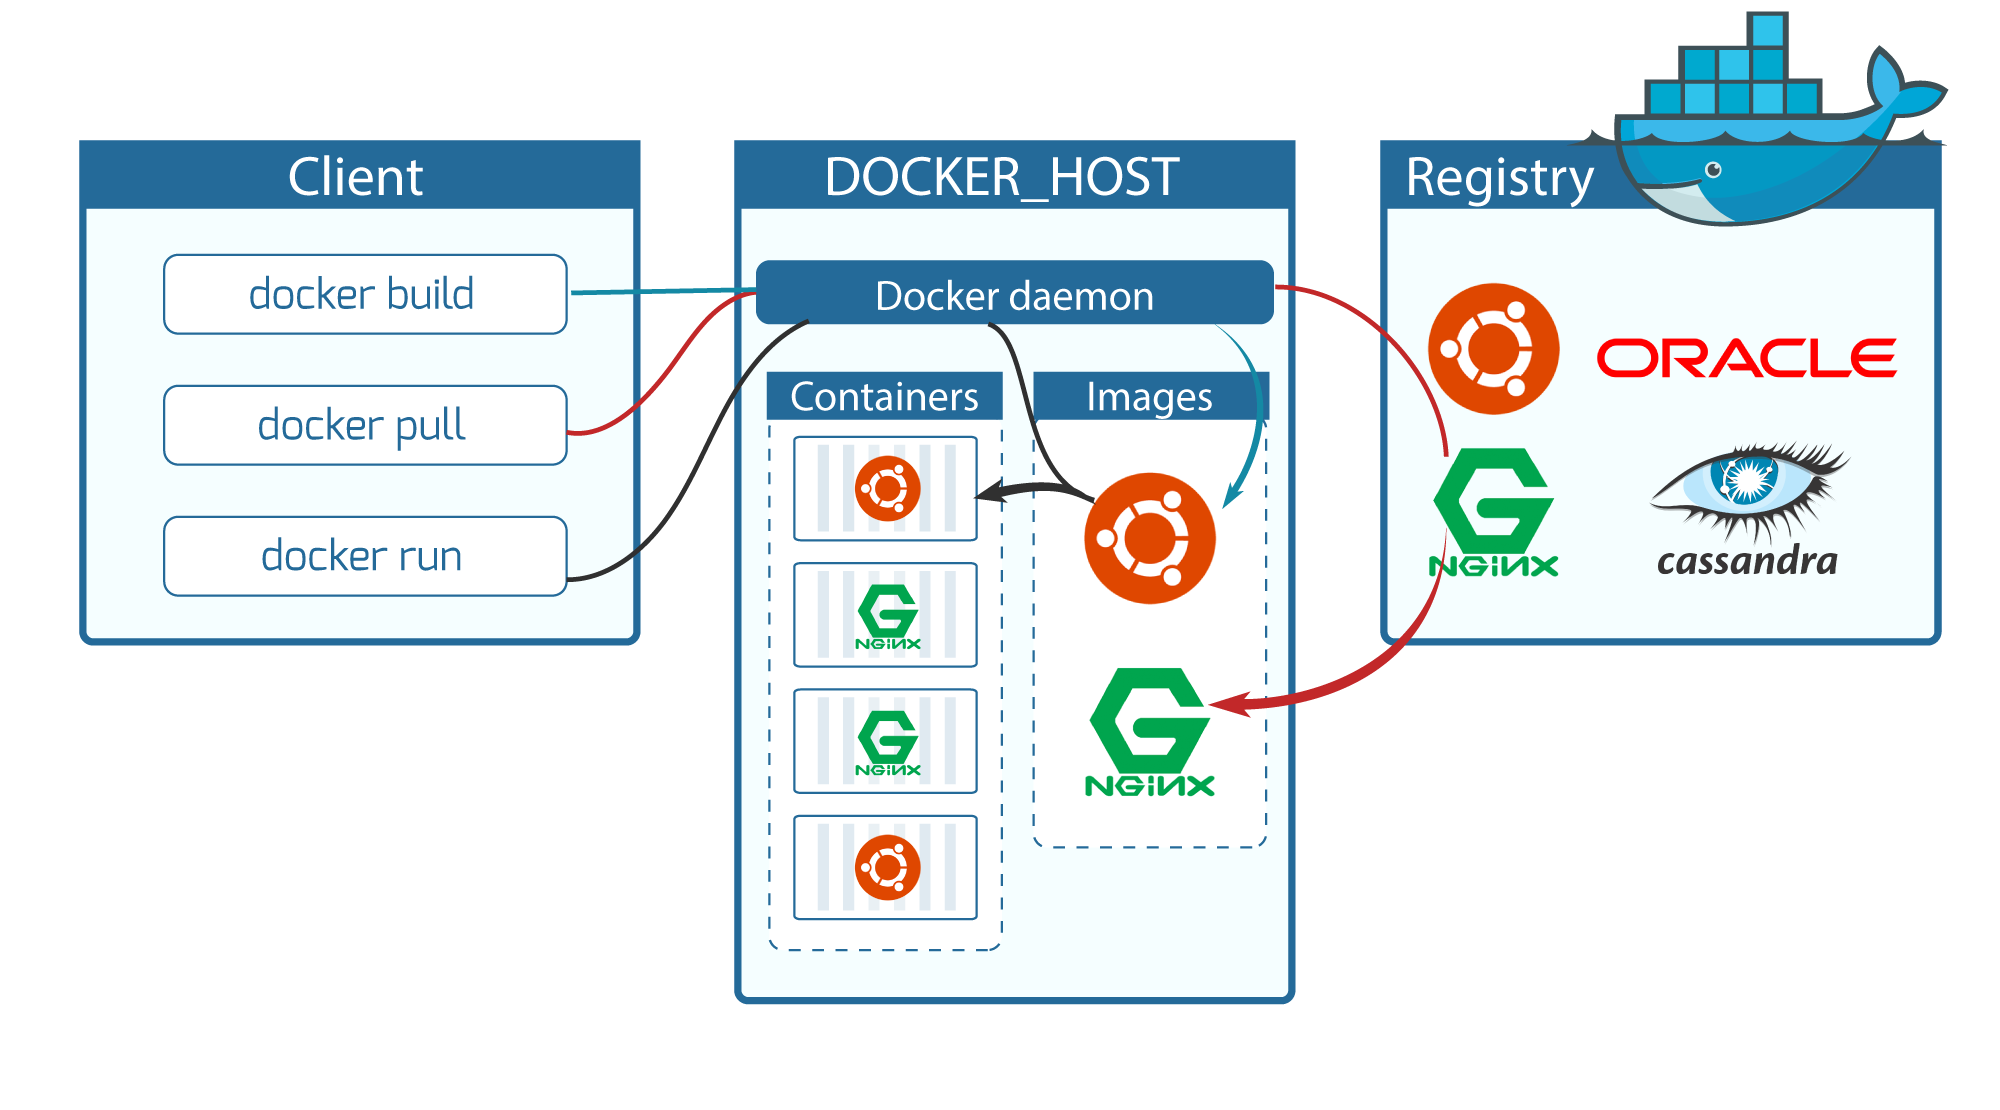
\includegraphics[width=\textwidth]{docker_architecture}
	\end{figure}
	De \textbf{Docker daemon} is verantwoordelijk om containers te starten, stoppen, monitoren, alsook om images op te slaan en te builden. De \textbf{Docker client} kan de daemon aanspreken om de operaties van de daemon uit te voeren. De \textbf{Registry} bevat images die door de daemon gebruikt kunnen worden.

	\underline{Een image aanmaken kan als volgt:}
	\begin{lstlisting}
# Dockerfile to build an Apache2 image
# Base image is Ubuntu
FROM ubuntu:14.04
# Install apache2 package
RUN apt-get update && apt-get install -y apache2 && apt-get clean
	\end{lstlisting}

	\underline{Syntax van een Dockerfile}:
	\begin{lstlisting}[numbers=left]
FROM ubuntu:14.04

COPY html /var/www/html
ADD web-page-config.tar /

ENV APACHE_LOG_DIR /var/log/apache
USER 73

EXPOSE 7373/udp 8080

RUN apt-get update && apt-get install -y \ apache 2 && apt-get clean

ENTRYPOINT ["echo", "Dockerfile entrypoint Demo"]
	\end{lstlisting}
	\begin{itemize}
		\item[\info] \textbf{Lijn 1 FROM} De base image van de container. Alle volgende commandos bouwen verder op deze image. 
		\item[\info] \textbf{Lijn 3 COPY} Bestanden kopieren van de docker host naar het bestandssysteem van de nieuwe image.
		\item[\info] \textbf{Lijn 4 ADD} Gelijkaardig aan COPY, maar kan ook .tar bestanden (die hij zal unzippen) en URLs (die hij zal downloaden) behandelen.
		\item[\info] \textbf{Lijn 6 ENV} Een omgevingsvariabele instellen in de nieuwe image.
		\item[\info] \textbf{Lijn 7 USER} Een gebruiker toevoegen met een specifiek UID. Deze UID wordt ook gebruikt in volgende RUN, CMD of ENTRYPOINT instructies.
		\item[\info] \textbf{Lijn 9 EXPOSE} Deze instructie \underline{informeert} enkel dat  deze poorten zullen gebruikt worden. Docker zal zelf deze poorten niet openzetten.
		\item[\info] \textbf{Lijn 11 RUN} Deze instructie bevat commando's die uitgevoerd moeten worden tijdens de buildfase. Het is beter om slechts één RUN instructie te hebben, omdat docker een nieuwe, read-only, laag aanmaakt voor elke instructie.
		\item[\info] \textbf{Lijn 13 ENTRYPOINT} Het startpunt van de applicatie. Als deze applicatie stopt, wordt de container ook automatisch gestopt.
	\end{itemize}

	Wanneer een container gestart wordt vanuit een image, dan zal Docker een extra, schrijfbare, laag toevoegen. Op deze laag kunnen dan nieuwe bestanden gezet worden. Als de container verwijderd wordt, zullen ook deze bestanden verwijderd worden. Op die manier kunnen dus verschillende containers, die toch dezelfde image hebben, aparte informatie bewaren. 

	\underline{Een container builden}:
$$\texttt{docker build -t dockerfile .}$$
	\chapter{Container orchestration}
	\underline{Drie functies van een orchestration framework}:
	\begin{enumerate}
		\item \textbf{Resource management}: Een groep van machines als één cluster beschouwen, zodat het lijkt alsof deze groep één proces is met zijn eigen CPU-, RAM- en volumegebruik.
		\item \textbf{Scheduling}: Het bepalen welke groep van containers op welke machine moet komen. De default werkwijze is om te kijken naar de systeemresources die een groep nodig heeft, en een daarbijhorende machine te vinden die deze systeemresources kan aanbieden.
		\item \textbf{Service management}: Het blootstelling van de container aan de externe wereld. Ook zal het framework ervoor zorgen dat er genoeg instanties van een bepaalde service zijn. Verder zal het framework load balancing implementeren tussen deze instanties.
	\end{enumerate}

	\section{Kubernetes}
	\underline{Kubernetes is een voorbeeld van een orchestration framework}.

	\begin{itemize}
		\item[\info] Een machine in een cluster kan \underline{twee vormen aannemen:}
		\begin{itemize}
			\item[\info] \textbf{Master:} deze machine beheert de cluster en bevat volgende componenten:
			\begin{itemize}
				\item Het bevat een \underline{API server}, die aangesproken kan worden door ontwikkelaars om de nodes aan te spreken.
				\item De \underline{scheduler} bepaalt op welke node een pod ($\equiv$ container, maar specifiek voor kubernetes) moet komen.
				\item De \underline{controller manager} is het proces dat verschillende kubernetes controllers bevat. Voorbeelden van controllers zijn:
				\begin{itemize}
					\item Replication Controller, die ervoor zorgt dat er een bepaald aantal kopieën van een pod aanwezig zijn in het cluster.
					\item Node Controller, die notificaties geeft wanneer een node niet meer bereikbaar is.
					\item Endpoints Controller, die pods en services samenvoegt.
				\end{itemize}
				\item Tot slot is er nog de \underline{etcd} storage, die configuratie en de staat van de cluster bewaart.
			\end{itemize}

			Meestal heeft een cluster maar een klein aantal masters.
			\item[\info] \textbf{Node:} Dit zijn de effectieve machines die de applicatie doen draaien en bevat volgende componenten:
			\begin{itemize}
				\item De \underline{kubelet} beheert de pods die aanwezig zijn op de node.
				\item De \underline{kube-proxy} voorziet een abstracte manier om de node te beheren.
				\item De \underline{cAdvisor} is een daemon that metrieken verzamelt.
				\item De \underline{pods} zijn de applicatieservices. 
			\end{itemize}
		\end{itemize}

		\item[\info] Een \underline{pod} is een eenheid van deployment in kubernetes, en bestaat uit één of meerdere containers die eenzelfde IP-adress en opslagvolume delen. Kubernetes maakt zelf de pods aan, met behulp van een document dat de gewenste staat beschrijft:
		\begin{lstlisting}
apiVersion: apps/v1beta1
kind: Deployment
metadata:
 name: myapp-deployment
spec:
 replicas: 3
 template:
  metadata:
   labels:
	app: MyApp
  spec:
   containers:
   - name: nginx
	 image: nginx:1.7.9
	 ports:
	 - containerPort:80
		\end{lstlisting}

		\item[\info] Vaak wordt er per pod maar één container geassocieerd, maar het is ook mogelijk om meerdere containers per pod te associeren. Dit is handig als je extra hulpfunctionaliteit wil bieden aan een service zoals:
		\begin{itemize} 
			\item[\info] \textbf{Sidecar container}: een service die periodiek een git pull doet om de applicatie up te daten. Een andere mogelijkheid is een service die logbestanden verwerkt.
			\item[\info] \textbf{Adapters}      
		\end{itemize}

		\item[\info] De \underline{service registry} is een databank van services, die voor elke service al zijn instanties en hun locaties bijhoudt. Een instantie wordt registreerd in de databank bij creatie, en wordt er terug uitgehaald bij destructie. clients moeten enkel nog aan de service registery een query doen, om de instanties op te halen voor een specifieke service. 
		\begin{itemize}
			\item[\info] \textbf{Client-side discovery}: Een client is gekoppeld aan de service registry en zal zelf load-balancing toepassen. Het nadeel is dat de client nu sterk gekoppeld is aan de service registry en dat er nu discovery logic in elke client aanwezig moet zijn.
			\item[\info] \textbf{Server-side discovery}: De client stuurt nu een request naar een load-balancer service, die op een bekende en vaste locatie ligt. De load-balancer zal nu zelf de service registry aanspreken en load-balancing implementeren. De client moet nu enkel een request sturen naar de load-balancer. Het nadeel is hier nu dat deze load-balancer opnieuw een component is dat moet onderhouden worden. Ook moet het gerepliceerd worden om beschikbaarheid te garanderen.
		\end{itemize}

		\item[\info] Kubernetes maakt gebruik van server-side discovery en vereist het aanmaken van een Kubernetes Service:
		\begin{lstlisting}
kind: Service
apiVersion: v1
metadata:
 name: myapp-service
spec:
 selector:
  app: MyApp
 ports:
 - protocol: TCP
   port: 8080
   target-port: 9000
		\end{lstlisting}
		Deze service zal clients een juiste pod bezorgen. 
	
		\item[\info] Een load balancer zal voor een bepaalde request bepalen welke instantie teruggeven moet worden. Enerzijds gebeurd dit op basis van de request, zoals bijvoorbeeld de geografische afstand, zodat enkel instanties in de omgeving relevant zijn. Anderzijds moet uit lijst van instanties degene gekozen worden op basis van de huidige capaciteit van een instantie.

		\item[\info] Er zijn \underline{drie interessante operaties} die uitgevoerd kunnen worden met een load balancer.
		\begin{enumerate}
			\item \textbf{Rolling update:} In plaats van elke instantie op hetzelfde moment up te daten, kan er altijd een selectie van instanties offline gehaald worden. De load-balancer stuurt dan de requests door naar de overige instanties.
			\item \textbf{Canary release:} Een kleine selectie van requests (bv 5\%) worden naar een instantie gestuurd die een nieuwe software update bevat. Op die manier worden weinig mensen getroffen door bugs, indien deze aanwezig zouden zijn.  
			\item \textbf{A/B testing:} Dit dient eerder voor marketingdoeleinden. De helft van de gebruikers krijgen versie A, en de andere helft krijgen versie B van een applicatie.
		\end{enumerate}
	\end{itemize}

	\section{Dimensies van cloud computing}
	\underline{Drie dimensies in cloud computing}
	\begin{itemize}
		\item[\info] Essentiële eigenschappen.
		\item[\info] Cloud service models.
		\item[\info] Cloud deployment models.
	\end{itemize}

	\subsection{Essentiële eigenschappen}
	\underline{vijf eigenschappen}
	\begin{itemize}
		\item[\info] \textbf{On-demand:} een resource moet op elk moment beschikbaar zijn.
		\item[\info] \textbf{Elasticiteit:} het aantal beschikbare resources moet instelbaar zijn, afhankelijk van de huidige nood.
		\item[\info] \textbf{Resource pooling:} De resources van de cloud provider worden gebruikt door meerder gebruikers. Een individuele gebruiker kan slechts op abstract niveau resources specificeren zoals het aanvragen van 6GB ram.
		\item[\info] \textbf{Metered:} Het gebruik van resources wordt in het oog gehouden. Meestal moet enkel voor de effectief gebruikte resources betaald worden.
		\item[\info] \textbf{Network access:} Een API is beschikbaar om de resources aan te spreken.
	\end{itemize}
	\subsection{Cloud service models}
	\underline{eerst stakeholders beschrijven}:
	\begin{itemize}
		\item[\info] \textbf{Cloud provider:} De provider beheert de hardware en software en stelt deze ter beschikking voor cloud users. De cloud provider is verantwoordelijk om de afgesproken requirements met de verschillende cloud users na te leven, meestal in de vorm van minimale garanties die de cloud provider moet leveren. Voorbeelden van cloud providers zijn: Amazon, Google en Microsoft.
		\item[\info] \textbf{Cloud users:} De cloud users gebruikt de resources van de cloud provider om applicaties te hosten, die dan gebruikt kunnen worden door end users. De cloud user heeft geen zicht op de interne structuur van de cloud provider, en kan enkel resources aanvragen. Er is geen formeel contract tussen cloud users en end users. Een voorbeeld van een cloud user is Netflix.
		\item[\info] \textbf{End users:} De end users maken gebruik van de cloud applicaties van de cloud users. Meestal is hier een bepaalde kost aan verbonden (jaarlijkse subscriptie).
	\end{itemize}

	\underline{vijf service models}
	\begin{itemize}
		\item[\info] \textbf{Metal as a Service:} Huren van fysieke servers, kabels en electriciteit. De provider helpt met het instaleren van onder andere een besturingssysteem, configuratie van VLANs en andere toestellen op het netwerk ontdekken.
		\item[\info] \textbf{Infrastructure as a Service:} Huren van virtuele machines, opslag en netwerkinfrastructuur. 
		\item[\info] \textbf{Container as a Service:} Huren van pregeconfigureerde orchestratieplatformen zoals Kubernetes.
		\item[\info] \textbf{Platform as a Service:} Huren van middleware producten zoals database management systemen, applicatieservers, message brokers, enz. 
		\item[\info] \textbf{Software as a Service:} Huren van software.
	\end{itemize}

	\subsection{Cloud deployment models}
	\underline{drie deployment models}
	\begin{itemize}
		\item[\info] \textbf{Public cloud:} Iedereen kan de systeemresources huren en gebruiken. 
		\item[\info] \textbf{Private cloud:}
		\item[\info] \textbf{Hybrid cloud:}
	\end{itemize}

	\section{Elastische schaling}
	\underline{twee vormen van schaling}
	\begin{itemize}
		\item[\info] \textbf{Statische schaling:} De systeembeheerder voert zelf een commando in om meer of minder resources te voorzien, meestal als het te laat is.
		\item[\info] \textbf{Elastische schaling:} Het systeem voorziet zelf schaling, in kleine intervallen, op basis van de huidige workload.
	\end{itemize}
	\underline{drie typen workloads}
	\begin{itemize}
		\item[\info] \textbf{Statische workload:} In dit geval is de werkload nagenoeg altijd dezelfde, zodat elastische schaling niet zo nuttig lijkt. Toch is het handig om, indien een machine faalt, snel een nieuwe machine werkend te hebben. Elastische schaling vergemakkelijkt dit proces. 
		\item[\info] \textbf{Periodieke workload:} Bij voorgedefinieerde pieken, zoals applicaties die enkel beschikbaar moeten zijn per dag, is het wel handig om elastische schaling te hebben. Bij statische schaling kan je vooraf genoeg resources voorzien, maar op normale momenten zijn er dan teveel resources beschikbaar, zodat er meer moet betaald worden.
		\item[\info] \textbf{Dynamische niet-periodieke workload:} Deze niet-periodieke workloads kunnen vooraf geweten zijn (ticketverkoop) of niet (opeens meer interesse in bepaalde website). 
	\end{itemize}

	Om \underline{elastische schaling} toe te passen kan men steunen op \underline{twee types}:
	\begin{itemize}
		\item[\alert] \textbf{Verticale schaling:} De bestaande infrastructuur uitbreiden (meer geheugen, CPU, harde schijven in nodes steken). Dit is geen goede techniek, omdat het neerschalen niet eenvoudig toelaat. Alle nieuwe hardware zou er dan uit moeten gehaald worden.
		\item[\good] \textbf{Horizontale schaling:} Nieuwe nodes voorzien die dezelfde infrastructuur hebben. Op deze manier kan zelfs de capaciteit van de grootste node overschreden worden.
	\end{itemize}

	


 
	\part{Distributed Data Storage \& Processing}
	\chapter{De uitdagingen van moderne data}
	Data-intensieve applicaties moeten rekening houden met volgende vier categorieën:
	\begin{itemize}
		\item \textbf{Volume.} De hoeveelheid opslag die over verschillende plaatsen moeten opgeslagen worden.
		\item \textbf{Velocity.} De snelheid waarop nieuwe informatie actueel wordt.
		\item \textbf{Variety.} De verschillende soorten types van data die bestaan. 
		\item \textbf{Veracity.} De betrouwbaarheid van de data. 
	\end{itemize}
	\chapter{Datamodellen}
	\section{Het relationeel model}
	\accentuate{zie cursus relationele gegevensbanken, belangrijk is om gewoon de nadelen te kennen zoals:}
	\begin{itemize}
		\item Er zou een brede tabel nodig zijn met honderden kolommen (waarvan de meeste dan NULL zijn) om bijvoorbeeld de producten van een winkel op te slaan. Elk product heeft diverse kenmerken die eigen zijn aan een bepaalde productcategorie.
		\item Men zou dit kunnen oplossen door een nieuwe tabel te maken per productcategorie, maar dit introduceert veel tabellen en relaties (te vergelijken met het verhogen van de normaalvorm).
	\end{itemize}
	\section{Het document model}
	Informatie in een document model wordt in een boomstructuur met one-to-many relaties opgeslagen, en is daarom dus perfect voor \underline{one-to-many relaties}. Een document wordt opgeslagen als één string, meestal in JSON of XML formaat, op deze manier volstaat één enkele query om een hele object, en zijn relaties op te vragen. 

	Een extreem voordeel van het document model is dat het geen restricties oplegt aan de data. Er kunnen twee producten zijn die in het systeem herkent worden als "Product" maar een andere interne structuur hebben. Het \underline{document model} wordt dus best \underline{gekenmerkt door}:
	\begin{itemize}
		\item Flexibiliteit in het schemamodel. Dit wordt ook wel "schema-on-read" genoemd aangezien de client niet op voorhand kan weten welke structuur het document zal hebben.
		\item Data lokaliteit. Hiermee wordt bedoeld dat een document als één enkelvoudige string wordt opgeslagen, en alle informatie zit dan ook in die string. Er is geen nood aan het join-of indexeringmechanisme. Een document wordt altijd in zijn geheel ingelezen, dit kan een nadeel zijn indien slechts een beperkt aantal informatie van dat document nodig is.
	\end{itemize}

	\section{Het graaf model}
	Het document model volstaat voor one-to-many relaties, maar is niet perfect voor \underline{many-to-many} of \underline{many-to-one relaties} want dan moeten er toch "joins" gedaan worden, maar dan op documenten. Het graaf model kent twee soorten:
	\begin{enumerate}
		\item Een normale graaf met knopen en verbindingen, die beiden attributen kunnen hebben.
		\item Een drievoudig model waarbij alle informatie opgeslagen wordt als: \texttt{SUBJECT $\rightarrow$ PREDICATE $\rightarrow$ OBJECT}
	\end{enumerate}
	Gekende graafalgoritmen kunnen toegepast worden op dit model. Het \underline{graaf model} heeft een aantal \underline{use cases}:
	\begin{itemize}
		\item \textbf{Transportnetwerk.} Een graaf is de geschikte manier om een wegennet voor te stellen.
		\item \textbf{Linkanalyse.} Het zoeken van objecten die gerelateerd zijn aan een ander object (bv vrienden van vrienden zoeken).
	\end{itemize}

	\section{Het kolomfamilie model}
	\todo{xxx}

	\chapter{Gedistribueerde informatie}
	Waarom is het belangrijk dat informatie op verschillende nodes beschikbaar is?
	\begin{itemize}
		\item \textbf{Schaalbaarheid:} Een toestel heeft maar een maximum aantal geheugen, opslagplaats en schijfoperaties per seconde. Meerdere nodes betekent dat de belasting kan verdeeld worden tussen de nodes.
		\item \textbf{Fouttolerantie:} Een reverse voorzien voor in het geval dat een andere node uitvalt.
		\item \textbf{Latency:} Nodes geografisch verspreiden zodat connecties vanuit andere continenten niet traag zijn.
	\end{itemize}
	Er wordt best gebruik gemaakt van het \underline{horizontaal schaalschema}. Dit heeft als voordeel dat er geen speciale hardware vereist is, en er gewoon machines kunnen bijgekocht worden indien dit nodig zou zijn.

	Er zijn \underline{twee belangrijke patronen} om data de distribueren:
	\begin{enumerate}
		\item \textbf{Replicatie:} Dit is eenvoudig alle data dupliceren op elke verschillende node, zodat ze allemaal dezelfde data bevatten. De \underline{voordelen} zijn: hoge databeschikbaarheid en fouttolerantietegen het uitvallen van een node door de redundantie van de informatie. Het \underline{nadeel} is: hoe moeten we ervoor zorgen dat alle nodes over dezelfde data beschikken (zie sectie \ref{sec:replicatie})? 
		\item \textbf{Partitionering (sharding):} De grote hoeveelheid data kan ook gepartitioneerd worden, zodat elke node zijn unieke verzameling van gegevens bevat. Partitionering heeft een aantal \underline{voordelen}: Elke partitie moet slechts zijn beperkte data behandelen. Hoe groter de dataset wordt, hoe minder operaties een bepaalde partitie zal moeten uitvoeren, aangezien er meer patitities zullen ingevoerd worden zodat de data meer verspreidt ligt over alle partities. Het \underline{nadeel} is: hoe kunnen we bepalen op welke node een bepaald stukje informatie moet komen. Idealiter heeft elke node dezelfde workload.
	\end{enumerate}
	In praktijk worden replicatie en partitionering gecombineerd. Eerst wordt partitionering toegepast, waarna deze partities ook nog gerepliceerd worden.

	\section{Replicatie}
	\label{sec:replicatie}
	Er zijn \underline{twee modellen} om aan replicatie te doen: het leader-follow model en het leaderless model. Een node die repliceerd wordt een replica genoemd.
	\subsection{Leader-Follower model}
	Dit model verloopt in drie stappen:
	\begin{enumerate}
		\item Een replica wordt tot leader gemaakt. Enkel op deze replica mogen er writeoperaties plaatsvinden.
		\item Elke andere replica is een follower. Elke keer dat de leader naar zijn schijf schrijft, zal de leader ook de gewijzigde data doorsturen, in de vorm van een \underline{replication log}, naar alle followers. Deze replication log bevat instructies dat elke follower moet ondernemen zodat ze de update juist kunnen uitvoeren.
		\item Een client kan een readoperatie zowel aan de leader als aan een follower aanvragen. 
	\end{enumerate}
	Deze manier garandueerd dat de followers \underline{ooit zullen convergeren} naar de juiste toestand.
	\subsection{Leaderless model}
\end{document}
